% Options for packages loaded elsewhere
\PassOptionsToPackage{unicode}{hyperref}
\PassOptionsToPackage{hyphens}{url}
%
\documentclass[
]{article}
\usepackage{lmodern}
\usepackage{stata}
\usepackage{amssymb,amsmath}
\usepackage{ifxetex,ifluatex}
\ifnum 0\ifxetex 1\fi\ifluatex 1\fi=0 % if pdftex
  \usepackage[T1]{fontenc}
  \usepackage[utf8]{inputenc}
  \usepackage{textcomp} % provide euro and other symbols
\else % if luatex or xetex
  \usepackage{unicode-math}
  \defaultfontfeatures{Scale=MatchLowercase}
  \defaultfontfeatures[\rmfamily]{Ligatures=TeX,Scale=1}
\fi
% Use upquote if available, for straight quotes in verbatim environments
\IfFileExists{upquote.sty}{\usepackage{upquote}}{}
\IfFileExists{microtype.sty}{% use microtype if available
  \usepackage[]{microtype}
  \UseMicrotypeSet[protrusion]{basicmath} % disable protrusion for tt fonts
}{}
\makeatletter
\@ifundefined{KOMAClassName}{% if non-KOMA class
  \IfFileExists{parskip.sty}{%
    \usepackage{parskip}
  }{% else
    \setlength{\parindent}{0pt}
    \setlength{\parskip}{6pt plus 2pt minus 1pt}}
}{% if KOMA class
  \KOMAoptions{parskip=half}}
\makeatother
\usepackage{xcolor}
\IfFileExists{xurl.sty}{\usepackage{xurl}}{} % add URL line breaks if available
\IfFileExists{bookmark.sty}{\usepackage{bookmark}}{\usepackage{hyperref}}
\hypersetup{
  pdftitle={Installing and Using the Michigan Graph Scheme},
  pdfauthor={Andy Grogan-Kaylor},
  hidelinks,
  pdfcreator={LaTeX via pandoc}}
\urlstyle{same} % disable monospaced font for URLs
\usepackage[margin=1 in]{geometry}
\usepackage{graphicx,grffile}
\makeatletter
\def\maxwidth{\ifdim\Gin@nat@width>\linewidth\linewidth\else\Gin@nat@width\fi}
\def\maxheight{\ifdim\Gin@nat@height>\textheight\textheight\else\Gin@nat@height\fi}
\makeatother
% Scale images if necessary, so that they will not overflow the page
% margins by default, and it is still possible to overwrite the defaults
% using explicit options in \includegraphics[width, height, ...]{}
\setkeys{Gin}{width=\maxwidth,height=\maxheight,keepaspectratio}
% Set default figure placement to htbp
\makeatletter
\def\fps@figure{htbp}
\makeatother
\setlength{\emergencystretch}{3em} % prevent overfull lines
\providecommand{\tightlist}{%
  \setlength{\itemsep}{0pt}\setlength{\parskip}{0pt}}
\setcounter{secnumdepth}{-\maxdimen} % remove section numbering

\title{Installing and Using the Michigan Graph Scheme}
\author{Andy Grogan-Kaylor}
\date{22 Feb 2021 13:14:40}

\begin{document}
\maketitle

\hypertarget{introduction}{%
\section{Introduction}\label{introduction}}

Stata provides the use of graph schemes that improve the overall look of
graphs.

See \texttt{help\ scheme}.

The \emph{Michigan graph scheme} makes use of official University of
Michigan colors.

\hypertarget{installation}{%
\section{Installation}\label{installation}}

Use of the \emph{Michigan graph scheme} depends on installation of the
`lean2' graph scheme developed by Svend Juul.

Type \texttt{findit\ lean2} and click through on the install links to
install \texttt{lean2}.

Then type \texttt{net\ from\ https://agrogan1.github.io/Stata} and click
the links to install.

\hypertarget{example-data}{%
\section{Example Data}\label{example-data}}

We are going to use the famous ``iris'' data collected by Edgar
Anderson.

\begin{stlog}
. 
. use "iris.dta", clear
{\smallskip}
. 
. summarize
{\smallskip}
    Variable {\VBAR}        Obs        Mean    Std. Dev.       Min        Max
\HLI{13}{\PLUS}\HLI{57}
Sepal_Length {\VBAR}        150    5.843333    .8280661        4.3        7.9
 Sepal_Width {\VBAR}        150    3.057333    .4358663          2        4.4
Petal_Length {\VBAR}        150       3.758    1.765298          1        6.9
 Petal_Width {\VBAR}        150    1.199333    .7622377         .1        2.5
     Species {\VBAR}        150           2    .8192319          1          3
{\smallskip}
. 
\end{stlog}

\hypertarget{histogram}{%
\section{Histogram}\label{histogram}}

\begin{stlog}
. 
. histogram Petal_Length, scheme(michigan)
(bin=12, start=1, width=.49166667)
{\smallskip}
. 
\end{stlog}



\begin{figure}
\centering
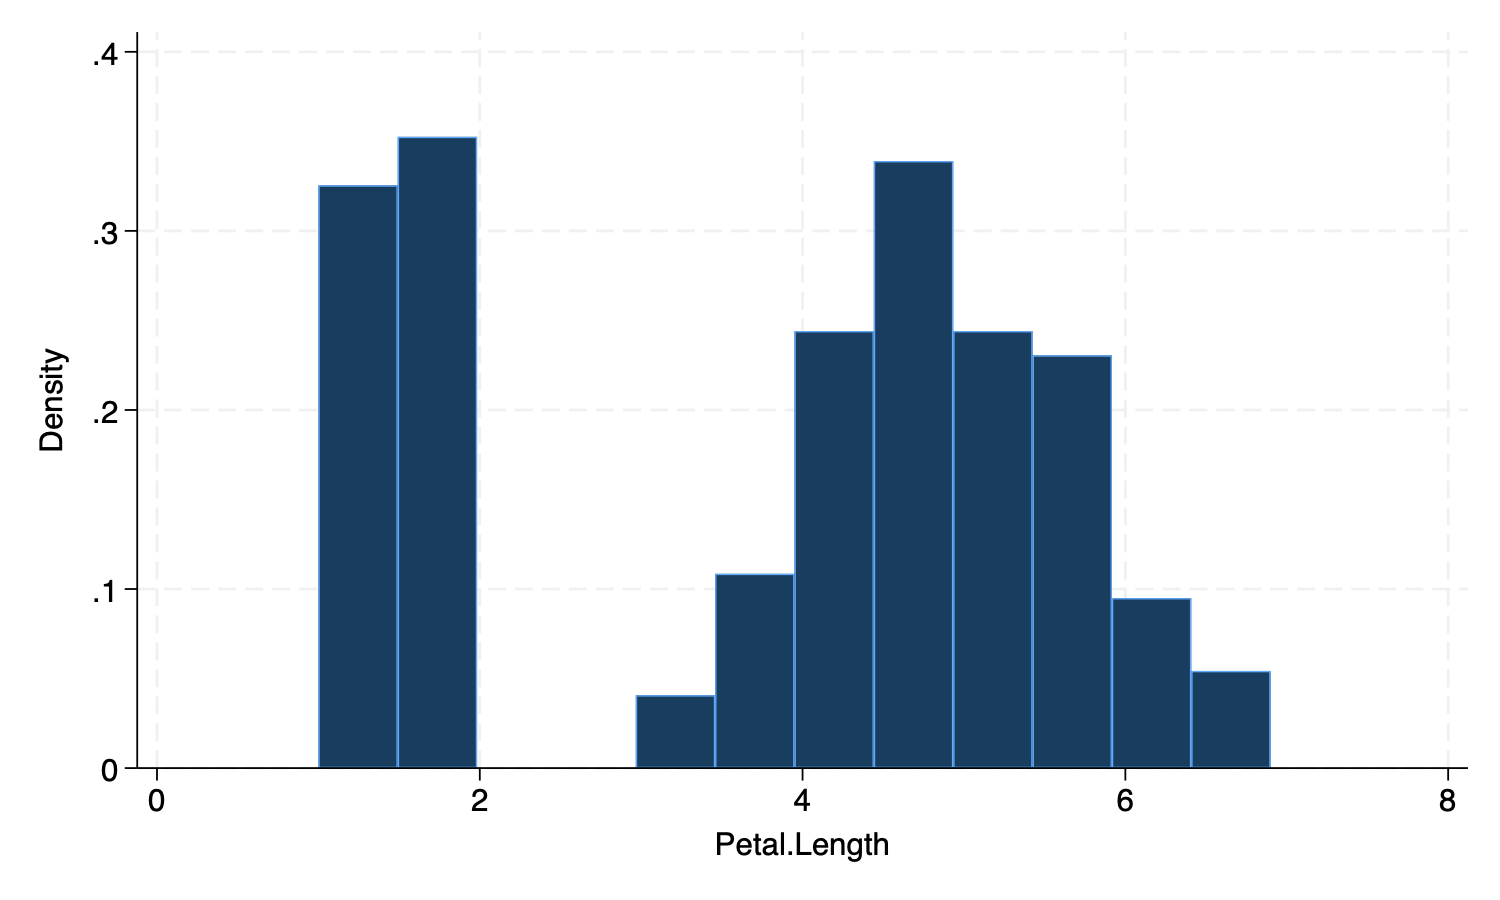
\includegraphics[width=0.75\linewidth]{myhistogram.png}
\caption{Histogram Using Michigan Scheme}
\end{figure}

\hypertarget{scatterplot}{%
\section{Scatterplot}\label{scatterplot}}

\begin{stlog}
. 
. twoway (scatter Petal_Length Petal_Width) ///
> (lfit Petal_Length Petal_Width), ///
> scheme(michigan)
{\smallskip}
. 
\end{stlog}



\begin{figure}
\centering
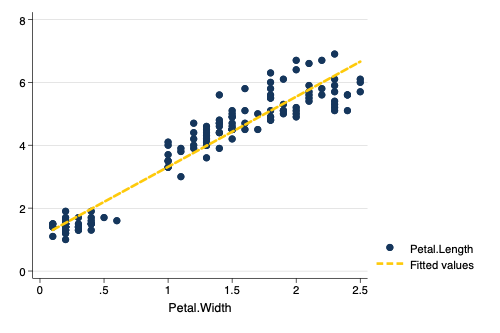
\includegraphics[width=0.75\linewidth]{myscatter.png}
\caption{Scatterplot Using Michigan Scheme}
\end{figure}

\end{document}
